\begin{frame}{Audiobooks on Storytel: Active Fanbase}
    \note{\tiny
    While I didn't have direct access to Storytel's actual listening data, I was able to leverage their publicly accessible datasets.
    By navigating through their app, I collated the number of reviews and average ratings for each book hosted on their platform.

    \begin{itemize}
    \item The scatterplot presented offers a comprehensive view of the engagement series has seen on Storytel.
    The y-axis showcases the number of reviews each book has accumulated to date (on logarithmic scale),
    while the x-axis delineates the release date of the audiobook.
    \item The data paints an interesting narrative: the series commenced with a robust 1104 reviews, tapering off to 395 by its culmination.
    It's reasonable to assume those who ventured into the last book had indeed perused the preceding titles.
    This gradient in reviews underscores a key behavior among readers: not everyone feels compelled to rate each book they consume.
    \item The overarching trend notwithstanding, the unwavering dedication of the series' fanbase is evident.
    The series holds a commendable median review count of 511 and never dips below 333 for any title.
    \item  Storytel's strategic rollout of the audiobooks was clearly well-thought-out — introducing a new chapter every Thursday,
    spaced out at intervals of 1 to 2 weeks across a 16-month duration.
    This systematic approach appears to be meticulously crafted not only to sustain audience engagement and heighten
    anticipation for upcoming releases but also to incentivize continuous subscription to their platform,
    ensuring listeners remain loyal and captivated over an extended period.
    \end{itemize}


    }
    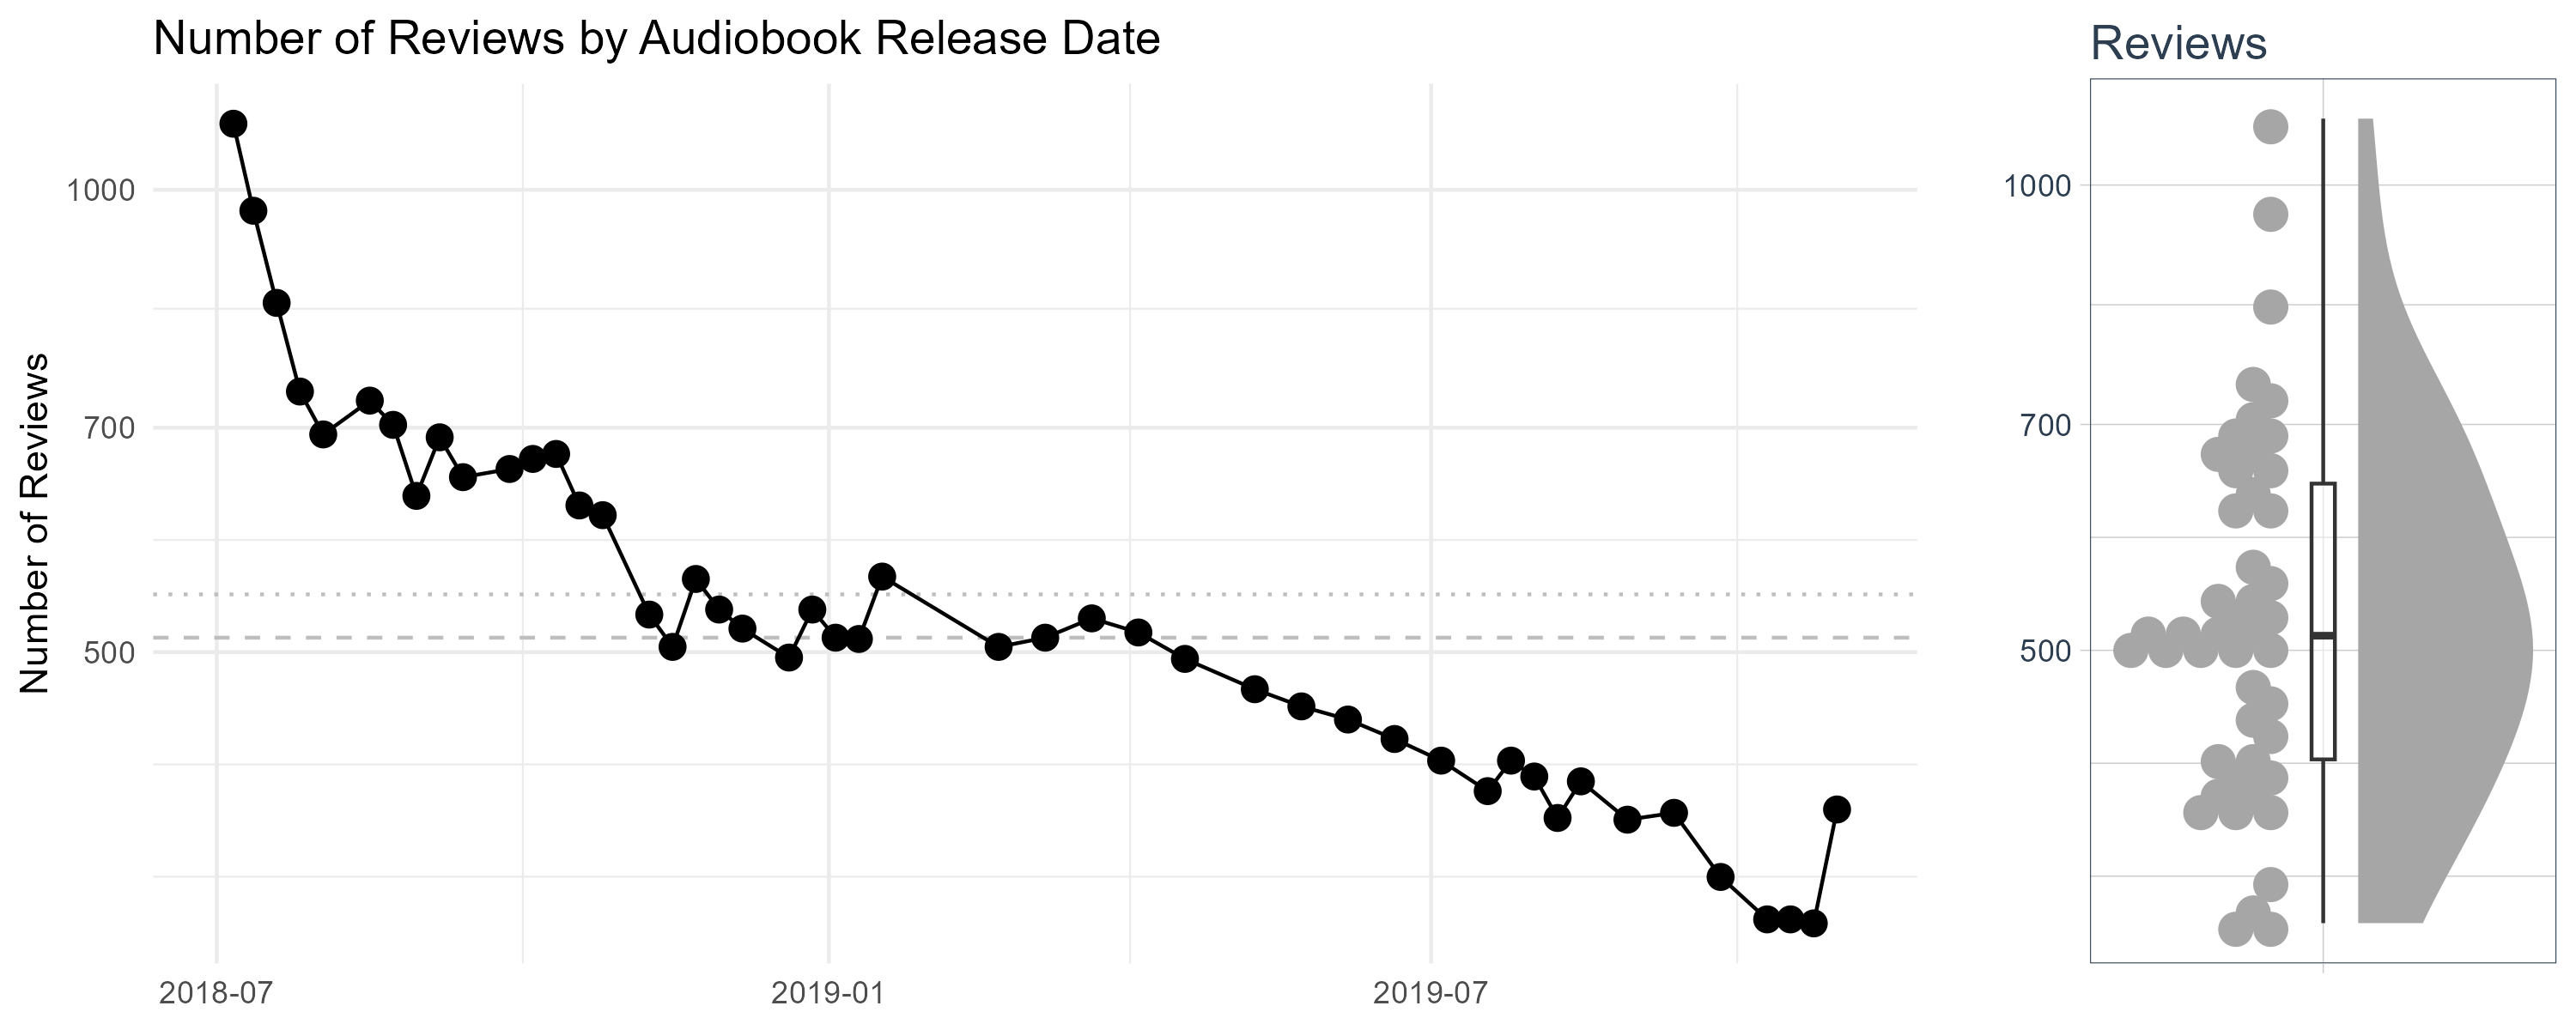
\includegraphics[width=\textwidth]{../rek-data-beers/R/figures/storytel_reviews}

    \begin{itemize}
    \item The series has a dedicated fanbase, with consistently high engagement.
    \item A solid median review count of 511, and minimum of 333.
    \item Releases on Thursdays, spaced 1--2 weeks apart, over 16-months.
    \end{itemize}

\end{frame}

\begin{frame}{Audiobooks on Storytel: High Ratings}
    \note{\scriptsize
    \begin{itemize}
    \item Similar to our earlier exploration, the y-axis on this plot represents the mean rating each title
    in the series has been awarded.

    \item The standout consistency is evident - with ratings ranging from a commendable 4.1 at their lowest,
    up to an impressive 4.6 stars - and median value settling at 4.5 stars.

    \item An important distinction to bear in mind is the merger of audiobook and e-book into a single entry on Storytel.
    This could make it challenging to differentiate if a review is based on the content of the book or the quality of the narration,
    potentially explaining some fluctuations in the ratings trend.

    \item Additionally, it's worth noting the dip in ratings observed in the latter part of the series.
    This aligns with Margit's own admissions of experiencing writer's fatigue during this period,
    which resulted in storylines that didn't quite live up to the standards set by the earlier entries in the series.
    It's a testament to the transparency of the author and the keen observation of her readers.
    \end{itemize}
    }

    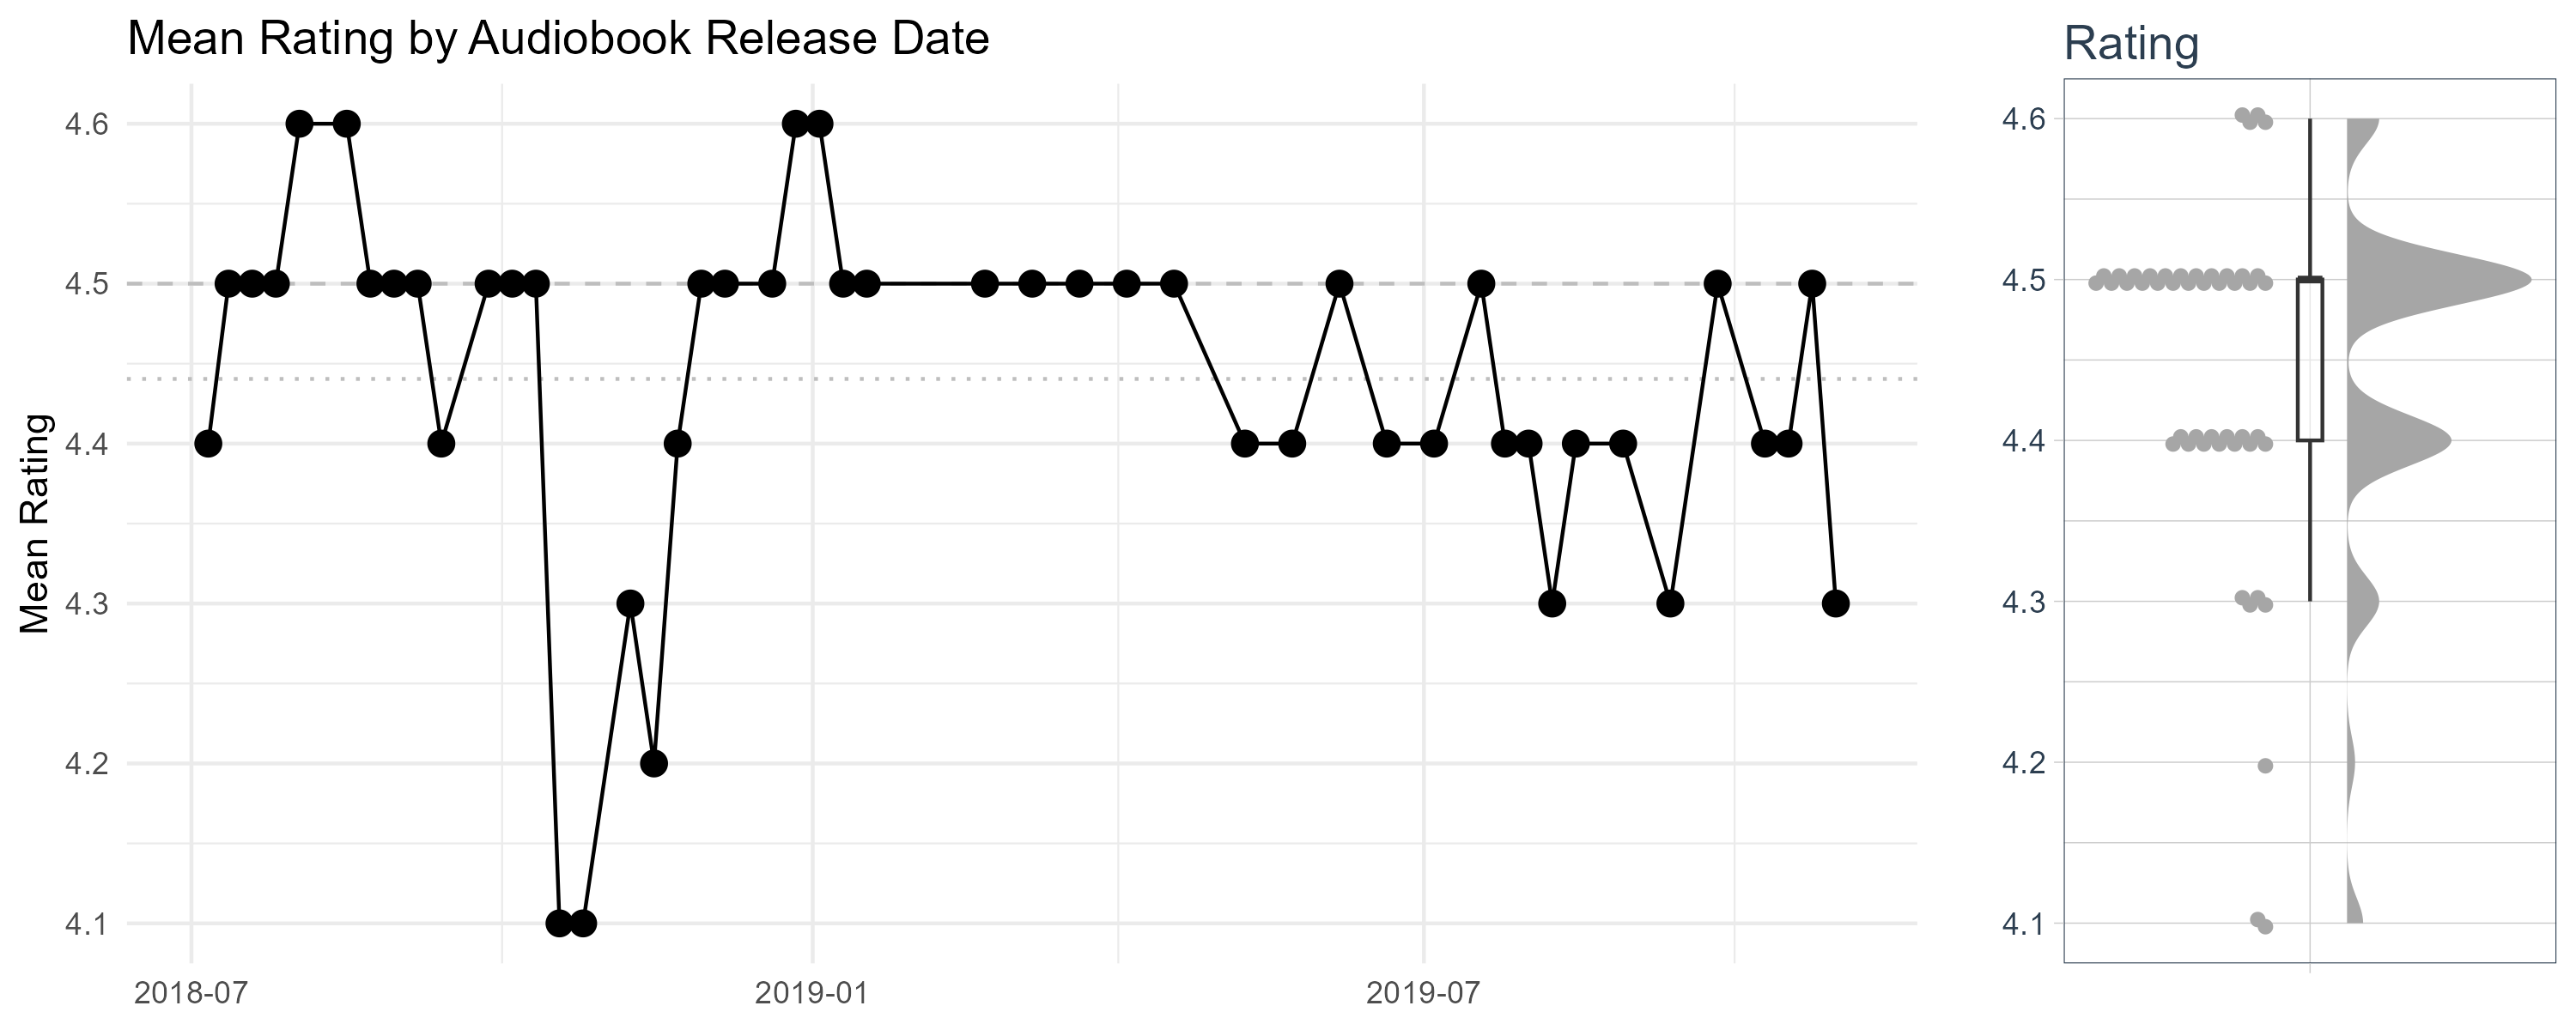
\includegraphics[width=\textwidth]{../rek-data-beers/R/figures/storytel_ratings}
    \begin{itemize}
    \item Overall high rating, an average 4.44 stars out of 5.
    \end{itemize}
\end{frame}

\begin{frame}{Audiobooks on Storytel: Our Narrators}
    \note{\tiny
    Let's pivot our attention to the narrators themselves, responsible for a whopping 18,000 minutes, or ~13 days, of continuous romantic medieval fantasy listening.

    On the chart, the y-axis now measures the total hours read per book.

    \begin{itemize}
    \item Intriguingly, although the books became shorter in written length as we observed earlier, their audiobook counterparts extended in duration. One might speculate if this `narration fatigue' implies that the readers began decelerating their reading pace over time.

    \item There's a circulating rumor that the initial narrator opted out of their contract after completing roughly a third of the series.
        The immersive narratives, challenging themes, including a pronounced emphasis on incestuous relationships and distressing topics like rape, might have taken a toll.

    \item The second narrator ambitiously aimed to provide each character with a unique voice.
        Given the vast array of characters introduced in the series, this quickly proved daunting.
        Their attempt at a radio-play narration style evidently wasn't well-received,
        as indicated by the subsequent drop in ratings shown in the slide before.
        While I'd wager that the content predominantly drives the ratings, shifts in narration styles can introduce variances.

    \item The third narrator adopted a more traditional narration style, leading ratings to return to their earlier levels. She handled nearly half of the series before handing over the reins.

    \item The dedication and adaptability of these narrators, each bringing their own unique flavor, are commendable and worth acknowledging.
    \end{itemize}
    }
    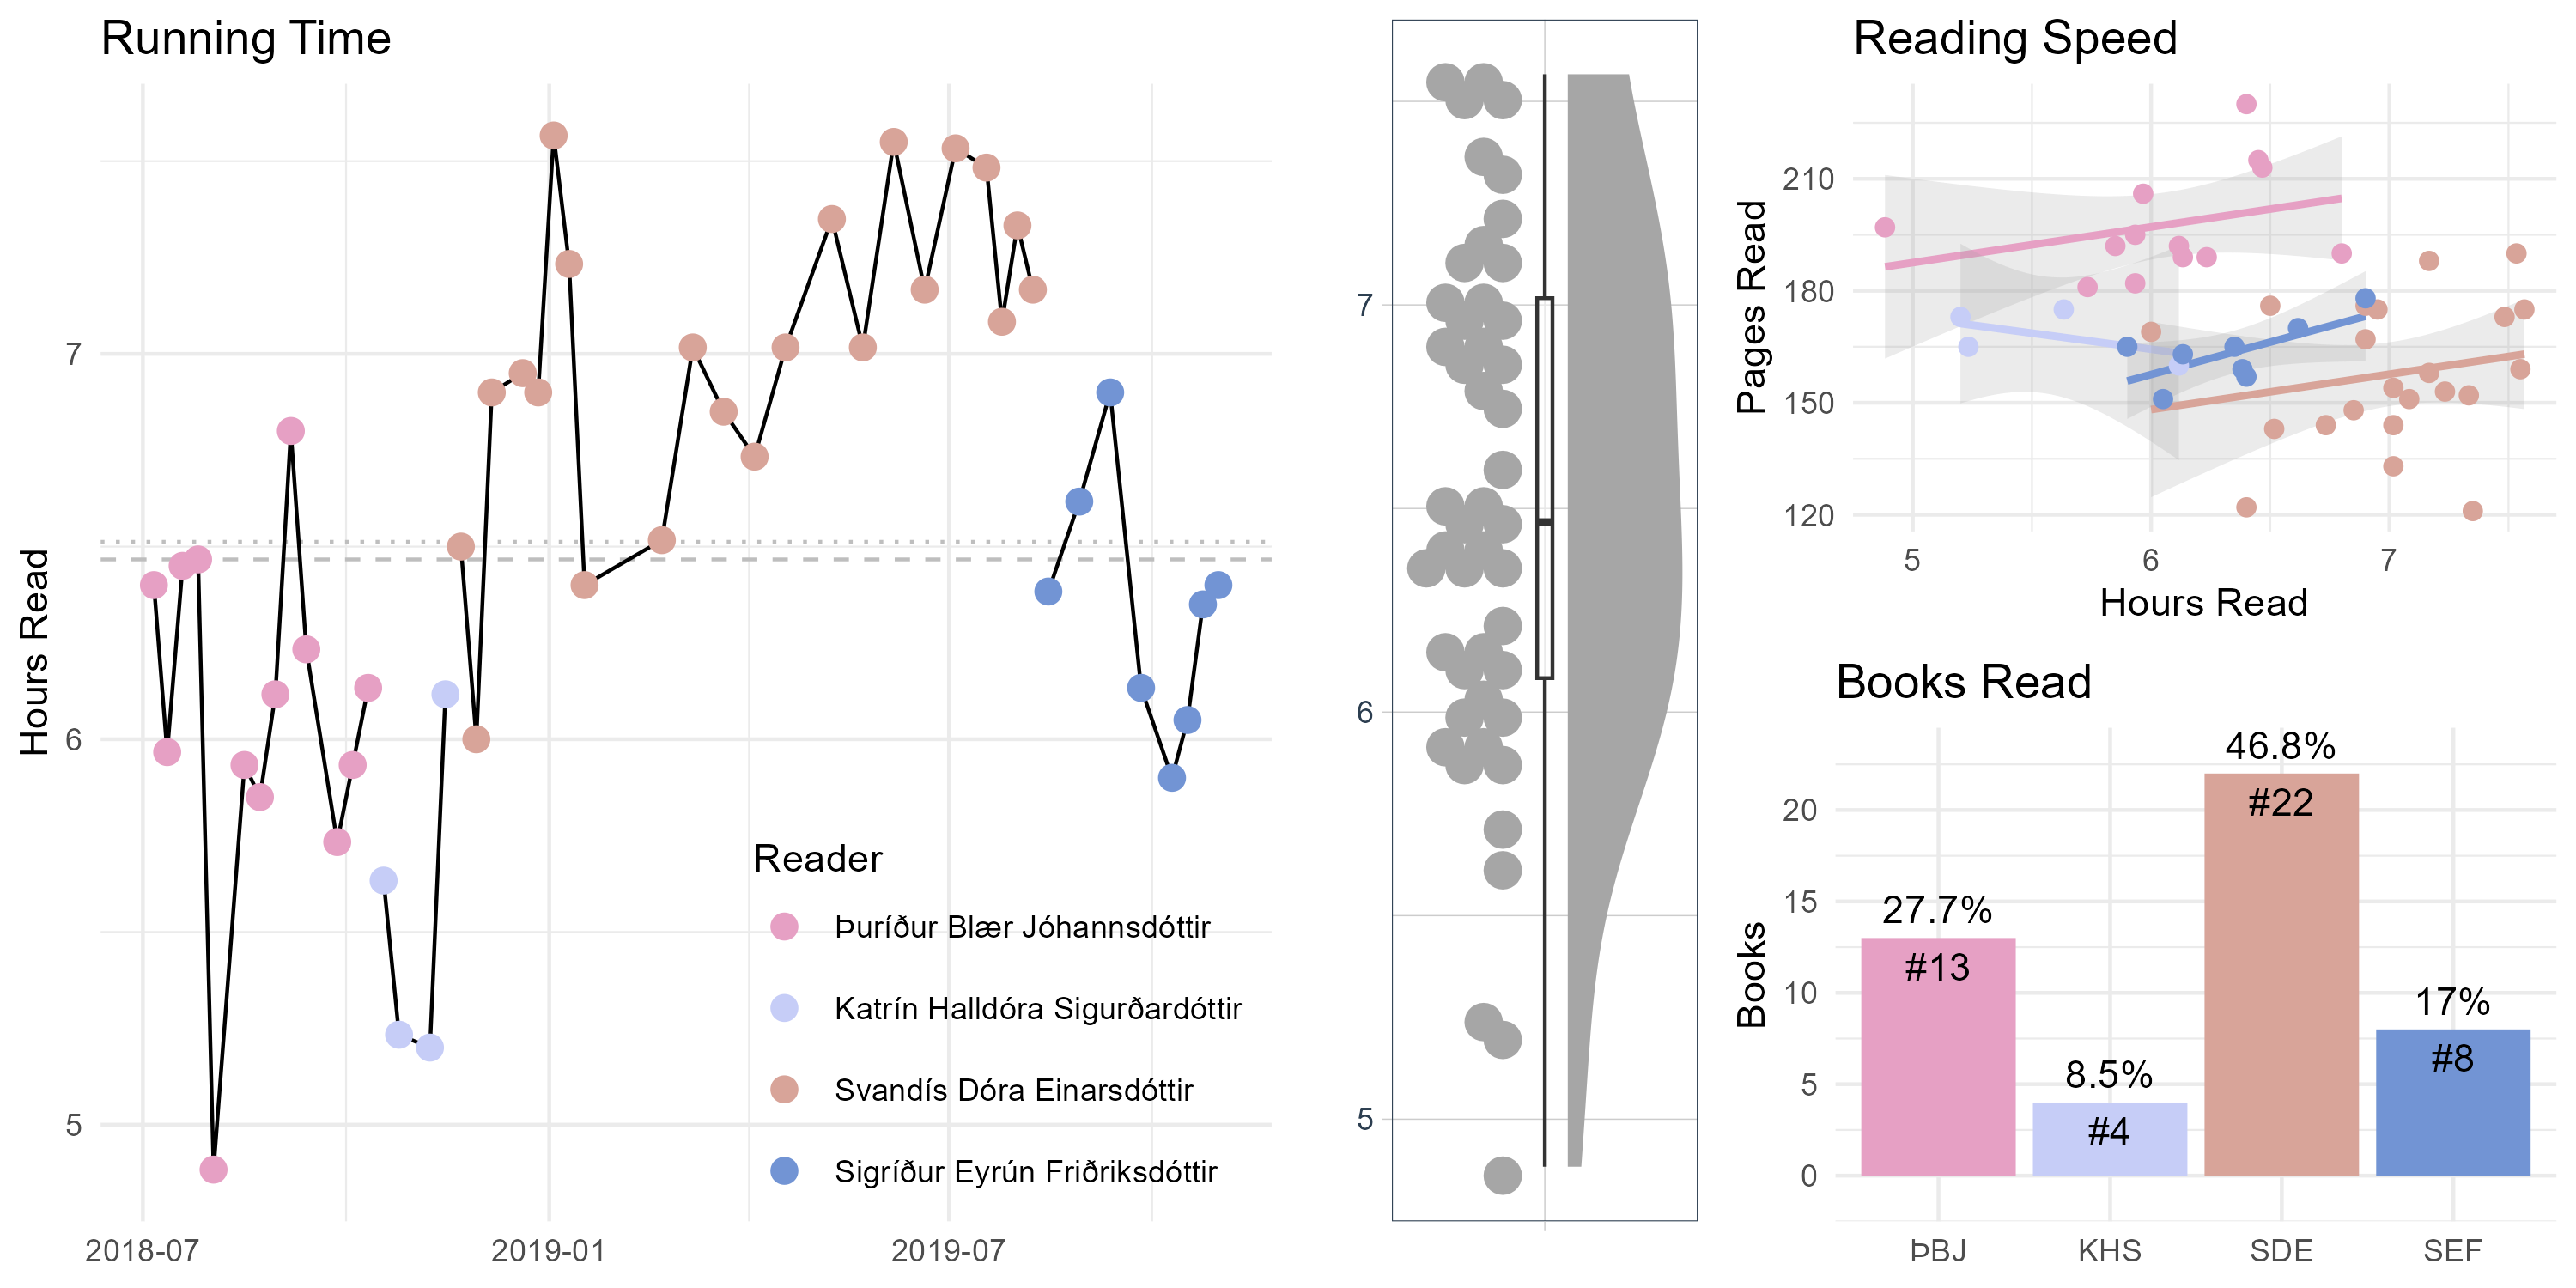
\includegraphics[width=\textwidth]{../rek-data-beers/R/figures/storytel_readers}
    \vspace{-18pt}
    \begin{itemize}
    \item Over 18K min of romantic medieval fantasy -- 12.8 days of cont. listening
    \item Four distinct voices with varied styles \& perseverance with Margit's prose
    \end{itemize}

\end{frame}
